\documentclass[class=book , crop=false]{standalone}

\usepackage{import} % Required for importing other .tex docs.  (import uses everything bw Begin and End Doc)
\usepackage{float} % Required for specifying the exact location of a figure or table
\usepackage{graphicx} % Required for including images
\usepackage{wrapfig}
\usepackage[pdftex,breaklinks,colorlinks=true,linkcolor=black,citecolor=blue,urlcolor=red,linktocpage=false,pagebackref=true,filecolor=magenta]{hyperref}%http://www.tug.org/applications/hyperref/manual.html#x1-100003.6
\usepackage{cite}
\usepackage[toc,title,page]{appendix}
\usepackage{pdfpages} % enables loading a pdf into the doc
\usepackage{makeidx}
\usepackage{glossaries} % must be after hyperref
\usepackage{blindtext}
\usepackage{enumitem}
%\usepackage{caption}

%\setlist[description]{leftmargin=\parindent,labelindent=\parindent}

%\renewcommand*{\bibname}{References} % renames the bibliography

\newcommand{\HRule}{\rule{\linewidth}{0.5mm}} % Command to make the lines in the title page

\graphicspath{{img/}{GIS_ChampionSection/img/}{awardsChapter/GIS_ChampionSection/img/}{brandPart/awardsChapter/GIS_ChampionSection/img/}{img/}{pairedProgSection/img/}{methodChapter/pairedProgSection/img/}{methodPart/methodChapter/pairedProgSection/img/}{documentationSection/img/}{methodChapter/documentationSection/img/}{methodPart/methodChapter/documentationSection/img/}{docStorageOrgSection/img/}{methodChapter/docStorageOrgSection/img/}{methodPart/methodChapter/docStorageOrgSection/img/}{QGisSection/img/}{toolsChapter/QGisSection/img/}{servicePart/toolsChapter/QGisSection/img/}{ESRISection/img/}{toolChapter/ESRISection/img/}{servicePart/toolChapter/ESRISection/img/}{../../../../source/}{../../source/}{servicePart/applicationsChapter/treasurerSection/img/}}

%\setlength\parindent{0pt} % eliminates indents

\newglossaryentry{ex}{name={sample},description={an example}}


\newglossaryentry{projection}{name={map projection},description={Representing a sphere on a flat surface}}
%\setcounter{tocdepth}{5}  % paragraph and down
\setcounter{tocdepth}{4}  % subparagraph and down
%\setcounter{tocdepth}{3}  % subsubsection and down

\def\titlename{Jalape\~no\\ \medskip\LARGE How This Book Works}

\title{\HRule % Horizontal Line added
\\[.4cm] % space
\begin{figure}[H] % included image
\begin{center}	% centered horizontally
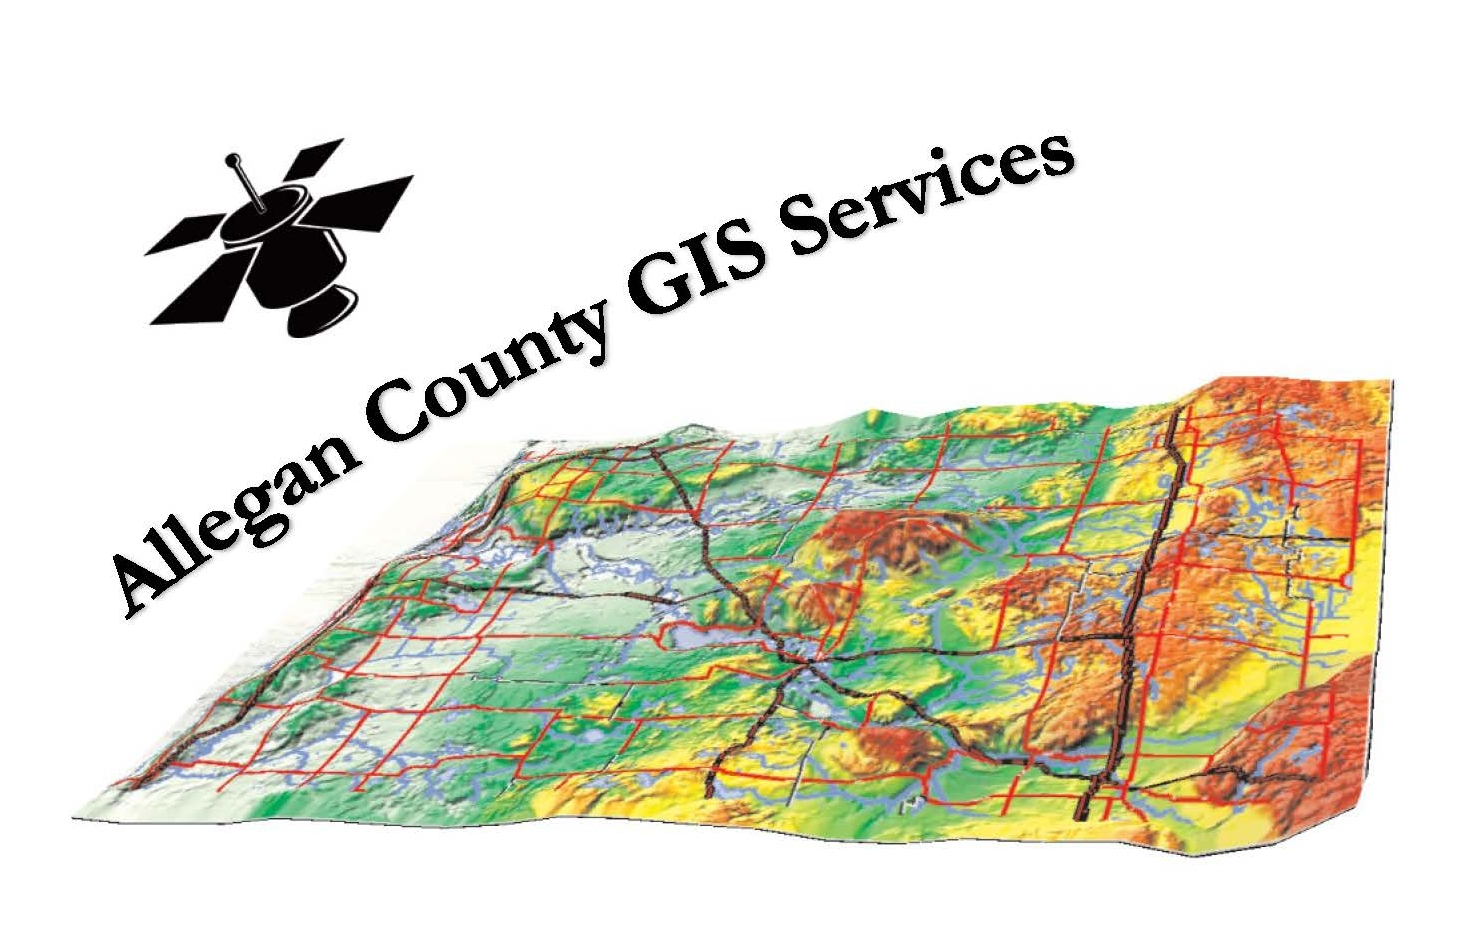
\includegraphics[scale=.45]{GIS_Logo_better.jpg}
\end{center}
\end{figure}
\Huge \bfseries \titlename \\ % Title text
\HRule \\[.4cm] % Horizontal Line added
\author{\Large Allegan County GIS \\\Large www.allegancounty.org/gis} % defines author
}  % closing brace for title

\begin{document}% Document Begins

\ifstandalone
\frontmatter % turns off chapter numbering and uses roman numerals for page numbers
\maketitle % creates title page and blank page after title page
\tableofcontents % creates TOC and blank page
\clearpage
\mainmatter % turns on chapter numbering, resets page numbering and uses arabic numerals for page numbers
\fi

\subsection[How Jalape\~no Works]{\large How \LARGE Jalape\~no \large Works}
\subsubsection{General Notes:}
\begin{itemize}
\item jalapeno folder is a git package.

\href{https://github.com/nbesteman/jalapeno}{https://github.com/nbesteman/jalapeno}

\item Project is coded with relative paths and jalapeno can be located anywhere.

\end{itemize}

\subsubsection{Project file structure:}
{\Large ...\textbackslash jalapeno\textbackslash..}\\
\begin{tabular}{p{4cm}| p{7cm} } 
%{\footnotesize folder & description} \\ \hline
folder & description \\ \hline 
documentation & resources used in Jalape\~no\\
processing & .tex douments and build folders\\
source & common image files\\
\end{tabular}
\bigskip\\
{\Large ...\textbackslash jalapeno\textbackslash documentation\textbackslash..}\\
\begin{tabular}{p{4cm} | p{7cm} } 
\footnotesize folder or file & description \\ \hline
moduleTemplates & .tex templates\\
packageDocs & \LaTeX{} documentation\\
references & reference and appendix resources\\
unsorted & catch all for unsorted documentation\\
BookStructureMM.mm & A mindmap of jalapeno\\
\end{tabular}
\bigskip\\
{\Large ...\textbackslash jalapeno\textbackslash processing\textbackslash..}\\
\begin{tabular}{p{4cm}| p{7cm} } 
\footnotesize folder or file & description \\ \hline
...Part & folders of book \textit{part}s\\
build & \LaTeX{} workspace and location of .pdf output and referenceEntries.bib* \\
commonTitle.tex & code for all title pages\\
fullCompile.sh & shell script to compile GISDocumentation.tex\\
GISDocumentation.tex & master document code\\
glossaryEntries.tex & entries that appear in glossary\\
indexEntries.tex & entries that appear in the index\\
preamble.tex & preamble code for all documents\\
\end{tabular}
\paragraph*{*Note about referenceEntries.bib}
{\footnotesize Any reference entries built here can be cited in any .tex document in the project.}

\subsubsection[Using the glossary]{{\Large Using the glossary}}
\paragraph{Glossary requirements:}
Glossary commands require a Perl interpreter.  Activeperl is a free Perl interpreter and can be downloaded from:\\ \href{https://www.activestate.com/activeperl/downloads}{https://www.activestate.com/activeperl/downloads}
{\tiny (A typical installation adds Perl to your path)}.  Compiling the glossary requires running the makeglossaries command either in a \LaTeX{} IDE or in command line as described here.  PDFLatex must be run first to create a .aux file that is used by makeglossaries to create an .gls file.  After the .gls file is created, PDFLatex must be run again to insert the glossary at the \textbackslash printglossaries location.
\paragraph{Creating a new glossary entry}
To \textbf{create a new glossary entry:} Add an entry to glossaryEntries.tex.  Save it there and then use the makeglossaries command to recompile the .gls file.
\paragraph{Rebuilding the glossary}
\textbf{To Recompile the .gls}.  In the (main document)build folder:
\begin{itemize}
\item Launch command prompt
\item enter command: \textbf{{\large makeglossaries GISDocumentation*}}
\end{itemize}
\subparagraph{*Note:} {\footnotesize This command reads the .aux file and creates the .gls file.  The .aux file is created by compiling with PDFLatex.  If there is no .aux file the command will fail.}
\paragraph{Using glossary terms in a subdocument:}
In the subdocument you must add code to input the glossaryEntries file.  For example:\\
After the line:
\begin{verbatim}
\usepackage{import} % Required for importing other .tex docs.  (import uses everything bw Begin and End Doc)
\usepackage{float} % Required for specifying the exact location of a figure or table
\usepackage{graphicx} % Required for including images
\usepackage{wrapfig}
\usepackage[pdftex,breaklinks,colorlinks=true,linkcolor=black,citecolor=blue,urlcolor=red,linktocpage=false,pagebackref=true,filecolor=magenta]{hyperref}%http://www.tug.org/applications/hyperref/manual.html#x1-100003.6
\usepackage{cite}
\usepackage[toc,title,page]{appendix}
\usepackage{pdfpages} % enables loading a pdf into the doc
\usepackage{makeidx}
\usepackage{glossaries} % must be after hyperref
\usepackage{blindtext}
\usepackage{enumitem}
%\usepackage{caption}

%\setlist[description]{leftmargin=\parindent,labelindent=\parindent}

%\renewcommand*{\bibname}{References} % renames the bibliography

\newcommand{\HRule}{\rule{\linewidth}{0.5mm}} % Command to make the lines in the title page

\graphicspath{{img/}{GIS_ChampionSection/img/}{awardsChapter/GIS_ChampionSection/img/}{brandPart/awardsChapter/GIS_ChampionSection/img/}{img/}{pairedProgSection/img/}{methodChapter/pairedProgSection/img/}{methodPart/methodChapter/pairedProgSection/img/}{documentationSection/img/}{methodChapter/documentationSection/img/}{methodPart/methodChapter/documentationSection/img/}{docStorageOrgSection/img/}{methodChapter/docStorageOrgSection/img/}{methodPart/methodChapter/docStorageOrgSection/img/}{QGisSection/img/}{toolsChapter/QGisSection/img/}{servicePart/toolsChapter/QGisSection/img/}{ESRISection/img/}{toolChapter/ESRISection/img/}{servicePart/toolChapter/ESRISection/img/}{../../../../source/}{../../source/}{servicePart/applicationsChapter/treasurerSection/img/}}

%\setlength\parindent{0pt} % eliminates indents

\end{verbatim}
Add the line:
\begin{verbatim}
\newglossaryentry{ex}{name={sample},description={an example}}


\newglossaryentry{projection}{name={map projection},description={Representing a sphere on a flat surface}}
\end{verbatim}
\subparagraph{To use a glossary term in the subdocument:\\}
In place of the term, use code referencing the key (in the glossaryEntries file):
\begin{itemize}
\item \textbackslash gls\{key\}
\end{itemize} 
\subparagraph{To add the glossary to the subdocument:}
\begin{itemize}
\item Add the line \textbackslash makeglossaries to the preamble of the subdocument.
\item Add the line \textbackslash printglossaries to the subdocument.
\item Run makeglossaries in command line on the subdocument similar to how is described above.
\end{itemize}




\subsubsection[Using the bibliography(References)]{{\Large Using the bibliography(References)}}
\paragraph{Bibliography requirements:}
Compiling the bibliography requires running bibtex either in a \LaTeX{} IDE or in command line as described here.  PDFLatex must be run first to create a .aux file that is used by bibtex to create a .bbl file.  After the .bbl file is created, PDFLatex must be run again to insert the bibliography at the \textbackslash bibliography location. \subparagraph{}
For example, the command:...\textbackslash bibliography\{referenceEntries\}\\
...places the bibliography called referenceEntries.bib which must be in the same folder as the project .aux file. 
\paragraph{Creating a new bibliography entry}
To \textbf{create a new bibliography entry:} Add an entry to referenceEntries.bib.  Save it there and then use bibtex to recompile the .bbl file.
\paragraph{Rebuilding the bibliography}
\textbf{To Recompile the .bbl}.  In the (main document)build folder:
\begin{itemize}
\item Launch command prompt
\item enter command: \textbf{{\large bibtex GISDocumentation}}
\end{itemize}
\subparagraph{*Note:} {\footnotesize This command reads the .aux file and creates the .bbl file.  The .aux file is created by compiling with PDFLatex.  If there is no .aux file the command will fail.}

\paragraph{To cite a bibliography source in a subdocument:} 
\subparagraph{}In the place that you want the citation:
\begin{itemize}
\item \begin{verbatim} ~\cite[pg.#]{key}\end{verbatim}
\end{itemize} 
\subparagraph{To add the bibliography to the subdocument:}
\begin{itemize}
\item Similar to adding to the master document but not documented here.
\end{itemize}


\subsubsection[Using the Index]{{\Large Using the Index}}
\paragraph{Index requirements:}
Compiling the index requires running the makeindex command either in a \LaTeX{} IDE or in command line as described here.  PDFLatex must be run first to create a .aux file that is used by makeindex to create an .idx file.  After the .idx file is created, PDFLatex must be run again to insert the index at the \textbackslash printindex location. 

\paragraph{Creating a new index entry}
To \textbf{create a new index entry:} Add an entry to indexEntries.tex.  Save it there and then use the makeindex command to recompile the .idx file.

\paragraph{Rebuilding the index}
\subparagraph{}\textbf{To Recompile the .idx}In the (main document)build folder:
\begin{itemize}
\item Launch command prompt
\item enter command: \textbf{{\large makeindex GISDocumentation*}}
\end{itemize}
\subparagraph{*Note:} {\footnotesize This command reads the .aux file and creates the .idx file.  The .aux file is created by compiling with PDFLatex.  If there is no .aux file the command will fail. Run PDFLatex first}

\paragraph{Using index terms in a subdocument:}
In the subdocument you must add code to input the indexEntries file.  For example:\\
After the line:
\begin{verbatim}
\usepackage{import} % Required for importing other .tex docs.  (import uses everything bw Begin and End Doc)
\usepackage{float} % Required for specifying the exact location of a figure or table
\usepackage{graphicx} % Required for including images
\usepackage{wrapfig}
\usepackage[pdftex,breaklinks,colorlinks=true,linkcolor=black,citecolor=blue,urlcolor=red,linktocpage=false,pagebackref=true,filecolor=magenta]{hyperref}%http://www.tug.org/applications/hyperref/manual.html#x1-100003.6
\usepackage{cite}
\usepackage[toc,title,page]{appendix}
\usepackage{pdfpages} % enables loading a pdf into the doc
\usepackage{makeidx}
\usepackage{glossaries} % must be after hyperref
\usepackage{blindtext}
\usepackage{enumitem}
%\usepackage{caption}

%\setlist[description]{leftmargin=\parindent,labelindent=\parindent}

%\renewcommand*{\bibname}{References} % renames the bibliography

\newcommand{\HRule}{\rule{\linewidth}{0.5mm}} % Command to make the lines in the title page

\graphicspath{{img/}{GIS_ChampionSection/img/}{awardsChapter/GIS_ChampionSection/img/}{brandPart/awardsChapter/GIS_ChampionSection/img/}{img/}{pairedProgSection/img/}{methodChapter/pairedProgSection/img/}{methodPart/methodChapter/pairedProgSection/img/}{documentationSection/img/}{methodChapter/documentationSection/img/}{methodPart/methodChapter/documentationSection/img/}{docStorageOrgSection/img/}{methodChapter/docStorageOrgSection/img/}{methodPart/methodChapter/docStorageOrgSection/img/}{QGisSection/img/}{toolsChapter/QGisSection/img/}{servicePart/toolsChapter/QGisSection/img/}{ESRISection/img/}{toolChapter/ESRISection/img/}{servicePart/toolChapter/ESRISection/img/}{../../../../source/}{../../source/}{servicePart/applicationsChapter/treasurerSection/img/}}

%\setlength\parindent{0pt} % eliminates indents

\end{verbatim}
Add the line:
\begin{verbatim}
% add index entries here and in the text for the index to track them
\index{map projections}
\index{ArcGIS Enterprise 10.5 functionality matrix}
\index{Portal Token}
\index{Token}
\index{coordinate systems}
\index{Michigan}
\index{State Plane}
\index{georef}
\index{State Tax Commission}
\index{Northing and Easting}
\index{PDF Optimization}
\index{File Rename}
\index{git Branching Model}
\index{PLSS}
\index{Town and Range}
\index{Township(Theoretiocal Diagram)}
\index{BLM}
\index{ANSI Paper}
\index{paper sizes}

\end{verbatim}

\subparagraph{To use a index term in the subdocument:\\}
In place of the term, use code referencing the key (in the indexEntries file):

\begin{itemize}
\item \textbackslash index \{key\}
\end{itemize} 

\subparagraph{To add the index to the subdocument:}
\begin{itemize}
\item Add the line \textbackslash makeindex to the preamble of the subdocument.
\item Add the line \textbackslash printindex to the subdocument.
\item Run makeindex in command line on the subdocument similar to how is described above.

\end{itemize}


\subsubsection[Using the Appendices]{{\Large Using the Appendices}}

\end{document}
